% Created by tikzDevice version 0.12.6 on 2023-12-21 06:05:16
% !TEX encoding = UTF-8 Unicode
\documentclass[tikz]{standalone}

\nonstopmode

\usepackage[fontset=fandol]{ctex}
\usepackage{amsfonts,mathrsfs,amssymb}
\begin{document}

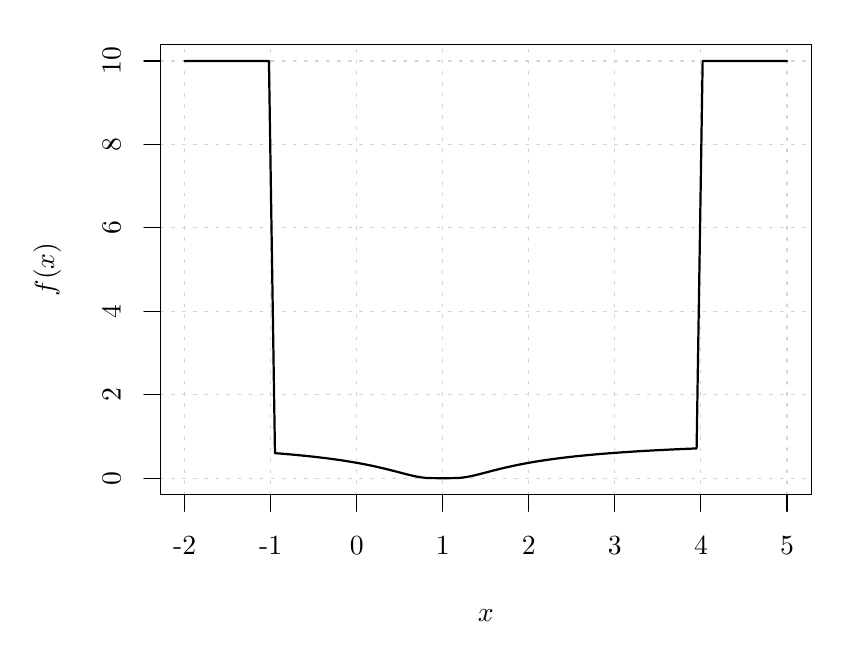
\begin{tikzpicture}[x=1pt,y=1pt]
\definecolor{fillColor}{RGB}{255,255,255}
\path[use as bounding box,fill=fillColor,fill opacity=0.00] (0,0) rectangle (289.08,216.81);
\begin{scope}
\path[clip] ( 48.00, 48.00) rectangle (283.08,210.81);
\definecolor{drawColor}{RGB}{211,211,211}

\path[draw=drawColor,line width= 0.4pt,dash pattern=on 1pt off 3pt ,line join=round,line cap=round] ( 56.71, 48.00) -- ( 56.71,210.81);

\path[draw=drawColor,line width= 0.4pt,dash pattern=on 1pt off 3pt ,line join=round,line cap=round] ( 87.80, 48.00) -- ( 87.80,210.81);

\path[draw=drawColor,line width= 0.4pt,dash pattern=on 1pt off 3pt ,line join=round,line cap=round] (118.90, 48.00) -- (118.90,210.81);

\path[draw=drawColor,line width= 0.4pt,dash pattern=on 1pt off 3pt ,line join=round,line cap=round] (149.99, 48.00) -- (149.99,210.81);

\path[draw=drawColor,line width= 0.4pt,dash pattern=on 1pt off 3pt ,line join=round,line cap=round] (181.09, 48.00) -- (181.09,210.81);

\path[draw=drawColor,line width= 0.4pt,dash pattern=on 1pt off 3pt ,line join=round,line cap=round] (212.18, 48.00) -- (212.18,210.81);

\path[draw=drawColor,line width= 0.4pt,dash pattern=on 1pt off 3pt ,line join=round,line cap=round] (243.28, 48.00) -- (243.28,210.81);

\path[draw=drawColor,line width= 0.4pt,dash pattern=on 1pt off 3pt ,line join=round,line cap=round] (274.37, 48.00) -- (274.37,210.81);

\path[draw=drawColor,line width= 0.4pt,dash pattern=on 1pt off 3pt ,line join=round,line cap=round] ( 48.00, 54.03) -- (283.08, 54.03);

\path[draw=drawColor,line width= 0.4pt,dash pattern=on 1pt off 3pt ,line join=round,line cap=round] ( 48.00, 84.18) -- (283.08, 84.18);

\path[draw=drawColor,line width= 0.4pt,dash pattern=on 1pt off 3pt ,line join=round,line cap=round] ( 48.00,114.33) -- (283.08,114.33);

\path[draw=drawColor,line width= 0.4pt,dash pattern=on 1pt off 3pt ,line join=round,line cap=round] ( 48.00,144.48) -- (283.08,144.48);

\path[draw=drawColor,line width= 0.4pt,dash pattern=on 1pt off 3pt ,line join=round,line cap=round] ( 48.00,174.63) -- (283.08,174.63);

\path[draw=drawColor,line width= 0.4pt,dash pattern=on 1pt off 3pt ,line join=round,line cap=round] ( 48.00,204.78) -- (283.08,204.78);
\definecolor{drawColor}{RGB}{0,0,0}

\path[draw=drawColor,line width= 0.8pt,line join=round,line cap=round] ( 56.71,204.78) --
	( 58.88,204.78) --
	( 61.06,204.78) --
	( 63.24,204.78) --
	( 65.41,204.78) --
	( 67.59,204.78) --
	( 69.77,204.78) --
	( 71.94,204.78) --
	( 74.12,204.78) --
	( 76.30,204.78) --
	( 78.47,204.78) --
	( 80.65,204.78) --
	( 82.83,204.78) --
	( 85.00,204.78) --
	( 87.18,204.78) --
	( 89.36, 63.06) --
	( 91.53, 62.89) --
	( 93.71, 62.71) --
	( 95.89, 62.52) --
	( 98.06, 62.31) --
	(100.24, 62.10) --
	(102.42, 61.87) --
	(104.59, 61.63) --
	(106.77, 61.37) --
	(108.95, 61.10) --
	(111.12, 60.80) --
	(113.30, 60.49) --
	(115.48, 60.15) --
	(117.65, 59.79) --
	(119.83, 59.41) --
	(122.01, 58.99) --
	(124.18, 58.55) --
	(126.36, 58.07) --
	(128.54, 57.57) --
	(130.71, 57.03) --
	(132.89, 56.48) --
	(135.07, 55.91) --
	(137.24, 55.35) --
	(139.42, 54.83) --
	(141.60, 54.40) --
	(143.77, 54.13) --
	(145.95, 54.04) --
	(148.13, 54.03) --
	(150.30, 54.03) --
	(152.48, 54.03) --
	(154.66, 54.05) --
	(156.83, 54.19) --
	(159.01, 54.51) --
	(161.19, 54.97) --
	(163.36, 55.50) --
	(165.54, 56.07) --
	(167.72, 56.64) --
	(169.89, 57.19) --
	(172.07, 57.72) --
	(174.25, 58.21) --
	(176.42, 58.68) --
	(178.60, 59.11) --
	(180.78, 59.52) --
	(182.95, 59.90) --
	(185.13, 60.25) --
	(187.31, 60.58) --
	(189.48, 60.89) --
	(191.66, 61.18) --
	(193.84, 61.45) --
	(196.01, 61.70) --
	(198.19, 61.94) --
	(200.37, 62.16) --
	(202.54, 62.37) --
	(204.72, 62.57) --
	(206.90, 62.76) --
	(209.07, 62.94) --
	(211.25, 63.10) --
	(213.43, 63.26) --
	(215.60, 63.41) --
	(217.78, 63.56) --
	(219.96, 63.70) --
	(222.13, 63.83) --
	(224.31, 63.95) --
	(226.49, 64.07) --
	(228.66, 64.18) --
	(230.84, 64.29) --
	(233.02, 64.40) --
	(235.19, 64.50) --
	(237.37, 64.59) --
	(239.55, 64.68) --
	(241.72, 64.77) --
	(243.90,204.78) --
	(246.08,204.78) --
	(248.25,204.78) --
	(250.43,204.78) --
	(252.61,204.78) --
	(254.78,204.78) --
	(256.96,204.78) --
	(259.14,204.78) --
	(261.31,204.78) --
	(263.49,204.78) --
	(265.67,204.78) --
	(267.84,204.78) --
	(270.02,204.78) --
	(272.20,204.78) --
	(274.37,204.78);
\end{scope}
\begin{scope}
\path[clip] (  0.00,  0.00) rectangle (289.08,216.81);
\definecolor{drawColor}{RGB}{0,0,0}

\path[draw=drawColor,line width= 0.4pt,line join=round,line cap=round] ( 56.71, 48.00) -- (274.37, 48.00);

\path[draw=drawColor,line width= 0.4pt,line join=round,line cap=round] ( 56.71, 48.00) -- ( 56.71, 42.00);

\path[draw=drawColor,line width= 0.4pt,line join=round,line cap=round] ( 87.80, 48.00) -- ( 87.80, 42.00);

\path[draw=drawColor,line width= 0.4pt,line join=round,line cap=round] (118.90, 48.00) -- (118.90, 42.00);

\path[draw=drawColor,line width= 0.4pt,line join=round,line cap=round] (149.99, 48.00) -- (149.99, 42.00);

\path[draw=drawColor,line width= 0.4pt,line join=round,line cap=round] (181.09, 48.00) -- (181.09, 42.00);

\path[draw=drawColor,line width= 0.4pt,line join=round,line cap=round] (212.18, 48.00) -- (212.18, 42.00);

\path[draw=drawColor,line width= 0.4pt,line join=round,line cap=round] (243.28, 48.00) -- (243.28, 42.00);

\path[draw=drawColor,line width= 0.4pt,line join=round,line cap=round] (274.37, 48.00) -- (274.37, 42.00);

\node[text=drawColor,anchor=base,inner sep=0pt, outer sep=0pt, scale=  1.00] at ( 56.71, 26.40) {-2};

\node[text=drawColor,anchor=base,inner sep=0pt, outer sep=0pt, scale=  1.00] at ( 87.80, 26.40) {-1};

\node[text=drawColor,anchor=base,inner sep=0pt, outer sep=0pt, scale=  1.00] at (118.90, 26.40) {0};

\node[text=drawColor,anchor=base,inner sep=0pt, outer sep=0pt, scale=  1.00] at (149.99, 26.40) {1};

\node[text=drawColor,anchor=base,inner sep=0pt, outer sep=0pt, scale=  1.00] at (181.09, 26.40) {2};

\node[text=drawColor,anchor=base,inner sep=0pt, outer sep=0pt, scale=  1.00] at (212.18, 26.40) {3};

\node[text=drawColor,anchor=base,inner sep=0pt, outer sep=0pt, scale=  1.00] at (243.28, 26.40) {4};

\node[text=drawColor,anchor=base,inner sep=0pt, outer sep=0pt, scale=  1.00] at (274.37, 26.40) {5};

\path[draw=drawColor,line width= 0.4pt,line join=round,line cap=round] ( 48.00, 54.03) -- ( 48.00,204.78);

\path[draw=drawColor,line width= 0.4pt,line join=round,line cap=round] ( 48.00, 54.03) -- ( 42.00, 54.03);

\path[draw=drawColor,line width= 0.4pt,line join=round,line cap=round] ( 48.00, 84.18) -- ( 42.00, 84.18);

\path[draw=drawColor,line width= 0.4pt,line join=round,line cap=round] ( 48.00,114.33) -- ( 42.00,114.33);

\path[draw=drawColor,line width= 0.4pt,line join=round,line cap=round] ( 48.00,144.48) -- ( 42.00,144.48);

\path[draw=drawColor,line width= 0.4pt,line join=round,line cap=round] ( 48.00,174.63) -- ( 42.00,174.63);

\path[draw=drawColor,line width= 0.4pt,line join=round,line cap=round] ( 48.00,204.78) -- ( 42.00,204.78);

\node[text=drawColor,rotate= 90.00,anchor=base,inner sep=0pt, outer sep=0pt, scale=  1.00] at ( 33.60, 54.03) {0};

\node[text=drawColor,rotate= 90.00,anchor=base,inner sep=0pt, outer sep=0pt, scale=  1.00] at ( 33.60, 84.18) {2};

\node[text=drawColor,rotate= 90.00,anchor=base,inner sep=0pt, outer sep=0pt, scale=  1.00] at ( 33.60,114.33) {4};

\node[text=drawColor,rotate= 90.00,anchor=base,inner sep=0pt, outer sep=0pt, scale=  1.00] at ( 33.60,144.48) {6};

\node[text=drawColor,rotate= 90.00,anchor=base,inner sep=0pt, outer sep=0pt, scale=  1.00] at ( 33.60,174.63) {8};

\node[text=drawColor,rotate= 90.00,anchor=base,inner sep=0pt, outer sep=0pt, scale=  1.00] at ( 33.60,204.78) {10};

\path[draw=drawColor,line width= 0.4pt,line join=round,line cap=round] ( 48.00, 48.00) --
	(283.08, 48.00) --
	(283.08,210.81) --
	( 48.00,210.81) --
	cycle;
\end{scope}
\begin{scope}
\path[clip] (  0.00,  0.00) rectangle (289.08,216.81);
\definecolor{drawColor}{RGB}{0,0,0}

\node[text=drawColor,anchor=base,inner sep=0pt, outer sep=0pt, scale=  1.00] at (165.54,  2.40) {$x$};

\node[text=drawColor,rotate= 90.00,anchor=base,inner sep=0pt, outer sep=0pt, scale=  1.00] at (  9.60,129.40) {$f(x)$};
\end{scope}
\end{tikzpicture}

\end{document}
